% !TeX root = ../thuthesis-example.tex

\chapter{内弹道的分析}

为了计算对应装药无侵蚀燃烧与有侵蚀燃烧时的发动机工作$p_{t}-t$曲线,我们需要先了解内弹道压力$p$的求解方式。根据参考资料\citep{tangjinlan}中的7.8节“一维侧面燃烧装药发动机内弹道的数值计算”,了解到我们可以根据以下微分方程组求得压力$p$等物理量。
\[
\frac{dp}{dx}=\frac{\rho u^2}{A_p}\frac{a^2}{a^2-u^2}\frac{dA_p}{dx}-\frac{\rho _pr\Pi u}{A_p}\left[ \frac{2a^2+\left( k-1 \right) u^2}{a^2-u^2} \right] 
\]
\[
\frac{du}{dx}=\frac{\rho _pr\Pi}{\rho A_p}\frac{a^2+ku^2}{a^2-u^2}-\frac{a^2u}{A_p\left( a^2-u^2 \right)}\frac{dA_p}{dx}
\]
\[
c_pT+\frac{u^2}{2}=c_pT_f
\]
\[
p=\rho RT
\]
\[
r=\overline{\varepsilon} ap^n
\]

$\Pi$——燃烧周界$\Pi =dA_b/dx$

$T_{f}$——绝热燃烧温度

$x$——观测位置距离圆心的距离

$a$——声速

$A_{b}$——燃面

由于能量守恒,通道中各截面的滞止温度$T_{0}$都是一样的,都等于$T_{f}$
\[
x=0,u_1=0
\]
\[
T_1=T_{01}=T_{\mathrm{f}}
\]
\[
p_1=\rho _1RT_1=p_{01}
\]
\[
x=L,\rho _Lu_LA_p=\frac{A_tp_{0L}}{c^*}
\]

显然,这里我们忽略了发动机燃烧室头部空腔和喷管前腔的影响。

\section{无侵蚀燃烧时的发动机工作$p_{t}-t$曲线}

\begin{figure}[H]
    \centering
    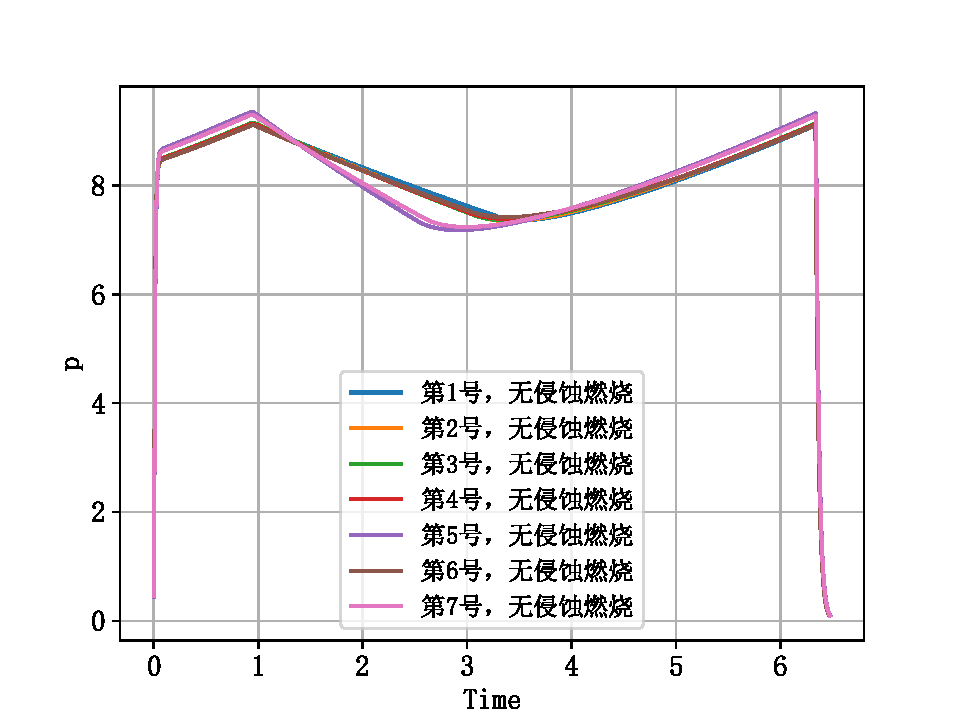
\includegraphics[width=0.89\linewidth]{无侵蚀燃烧全局图.pdf}
    \caption{无侵蚀燃烧全局图}
    \label{fig:example}
  \end{figure}
\vspace{1em}
\begin{figure}[!h]
    \centering
    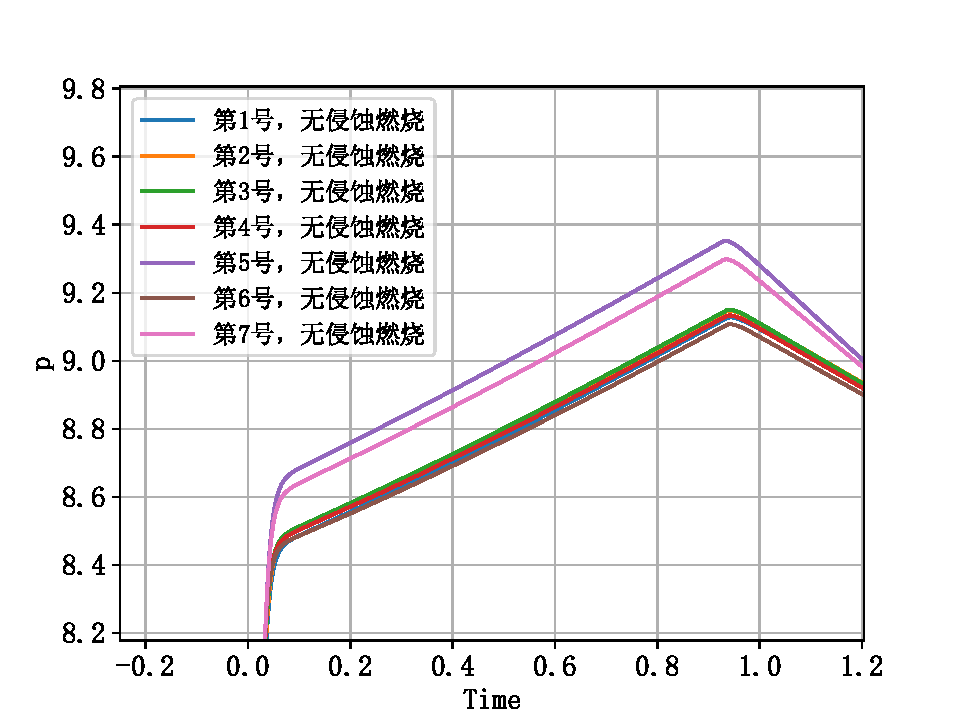
\includegraphics[width=0.89\linewidth]{无侵蚀燃烧局局图左.pdf}
    \caption{无侵蚀燃烧局部图(左)}
    \label{fig:example}
  \end{figure}

\begin{figure}[!h]
    \centering
    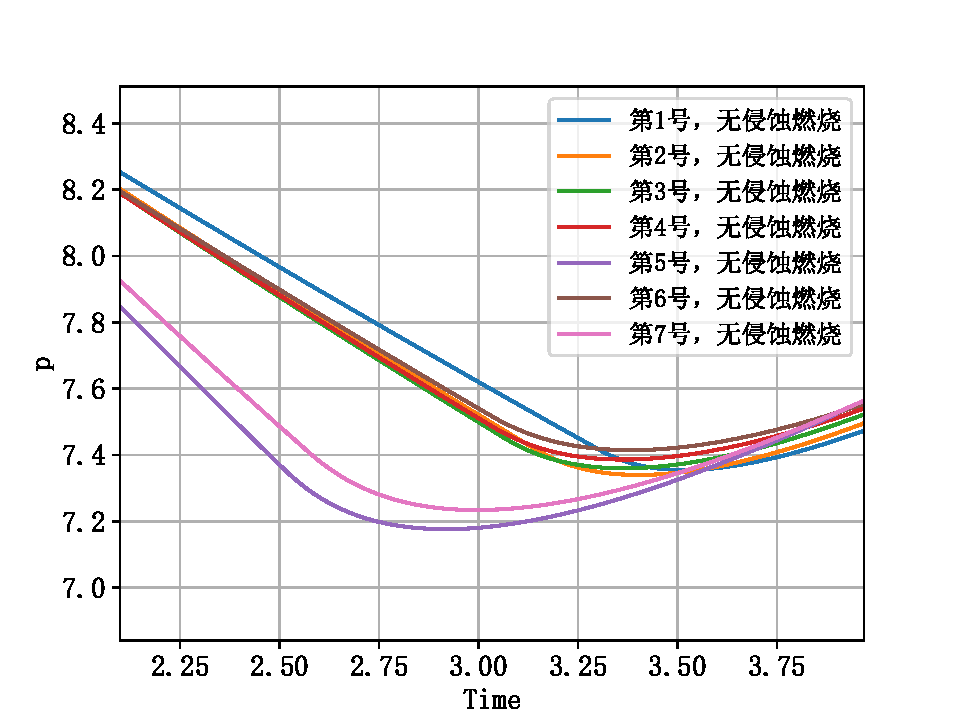
\includegraphics[width=1\linewidth]{无侵蚀燃烧局局图中.pdf}
    \caption{无侵蚀燃烧局部图(中)}
    \label{fig:example}
  \end{figure}

  \begin{figure}[!h]
    \centering
    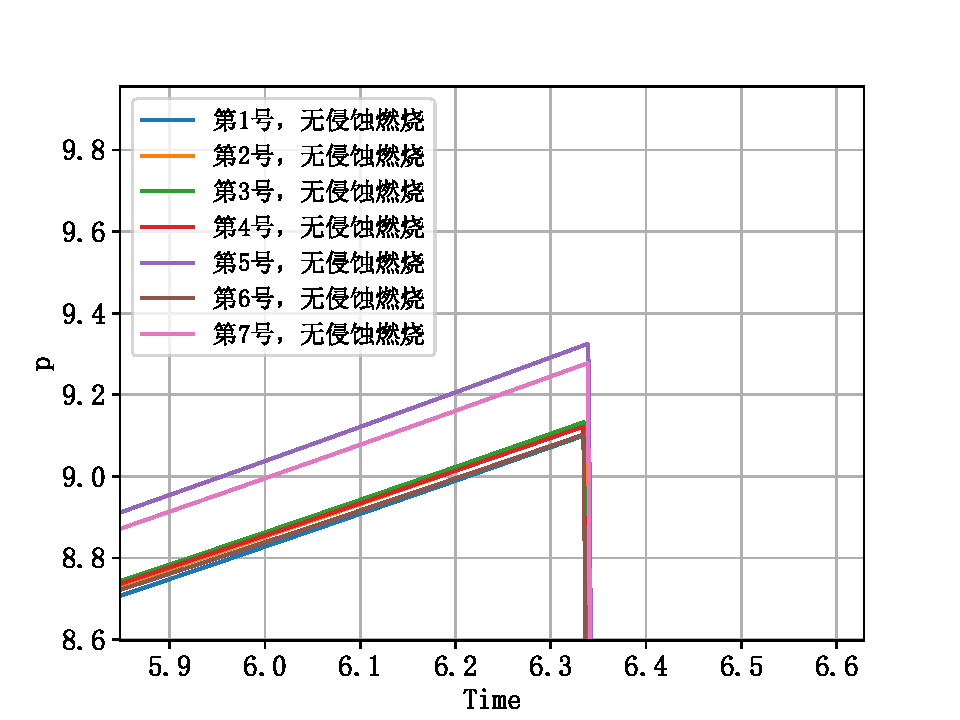
\includegraphics[width=1\linewidth]{无侵蚀燃烧局局图右.pdf}
    \caption{无侵蚀燃烧局部图(右)}
    \label{fig:example}
  \end{figure}

\section{有侵蚀燃烧时的发动机工作$p_{t}-t$曲线}

\begin{figure}[H]
    \centering
    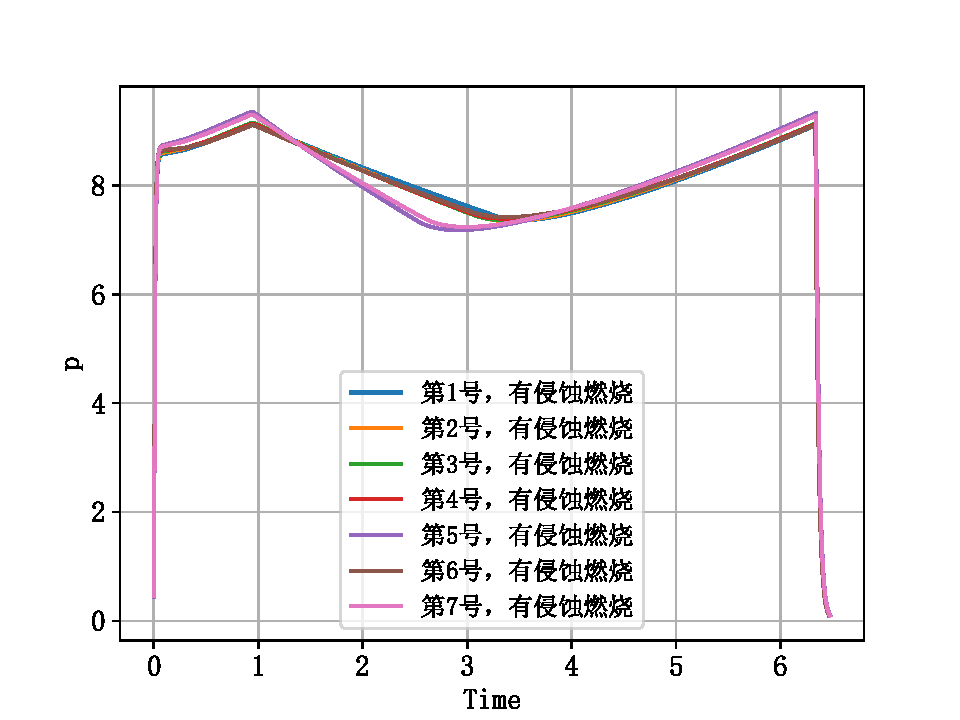
\includegraphics[width=0.89\linewidth]{有侵蚀燃烧全局图.pdf}
    \caption{有侵蚀燃烧全局图}
    \label{fig:example}
  \end{figure}

\begin{figure}[!h]
    \centering
    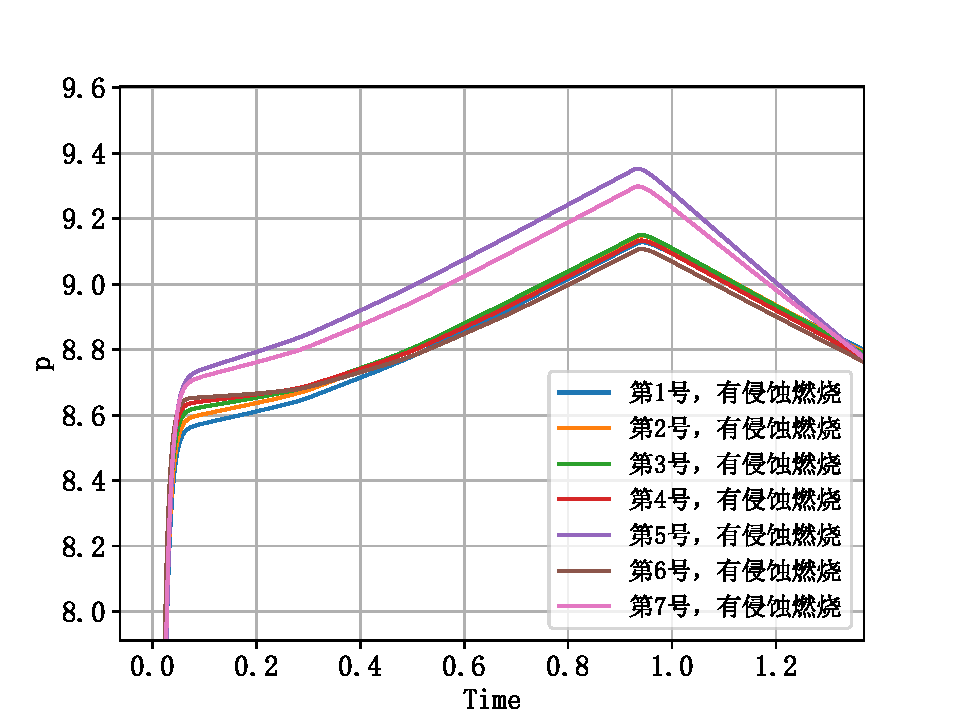
\includegraphics[width=0.89\linewidth]{有侵蚀燃烧局局图左.pdf}
    \caption{有侵蚀燃烧局部图(左)}
    \label{fig:example}
  \end{figure}

\begin{figure}[!h]
    \centering
    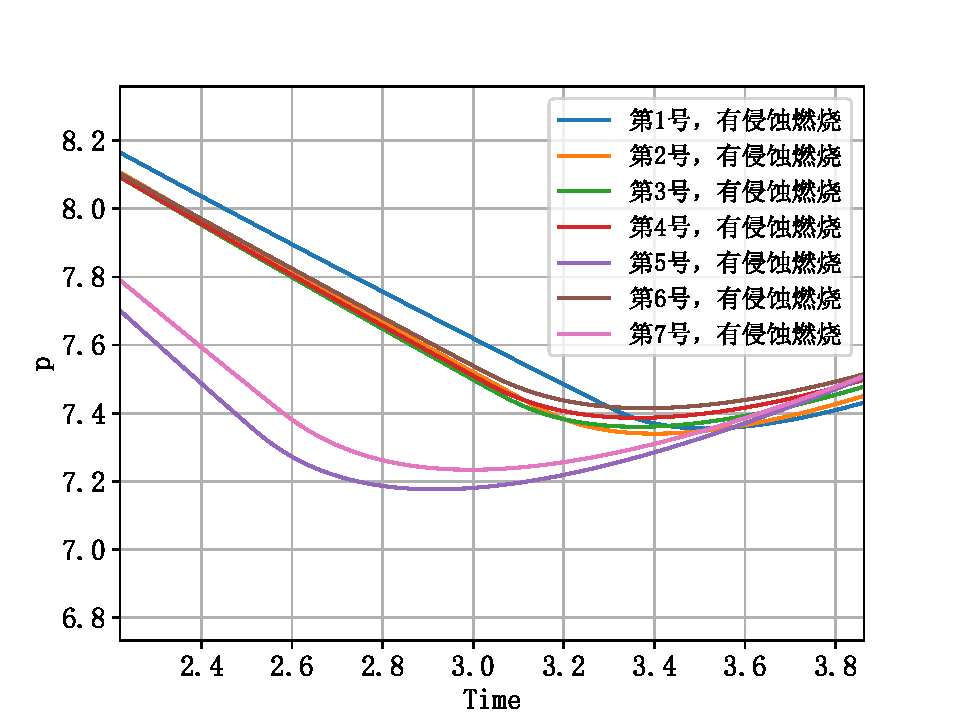
\includegraphics[width=1\linewidth]{有侵蚀燃烧局局图中.pdf}
    \caption{有侵蚀燃烧局部图(中)}
    \label{fig:example}
  \end{figure}

  \begin{figure}[!h]
    \centering
    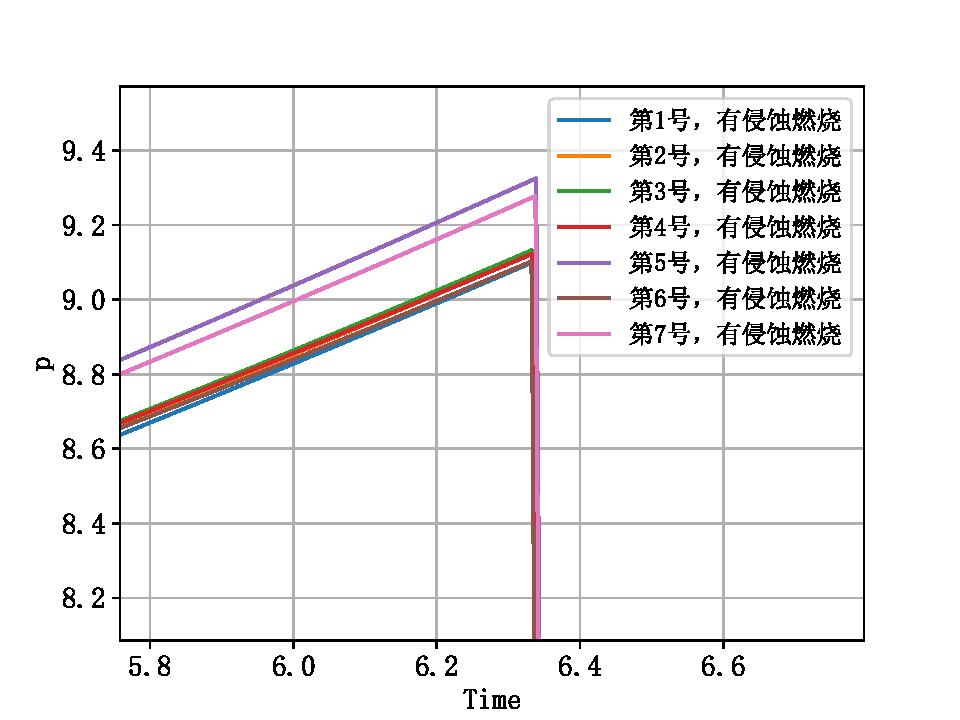
\includegraphics[width=1\linewidth]{有侵蚀燃烧局局图右.pdf}
    \caption{有侵蚀燃烧局部图(右)}
    \label{fig:example}
  \end{figure}

\section{无侵蚀燃烧与有侵蚀燃烧对比}
\begin{figure}[H]
    \centering
    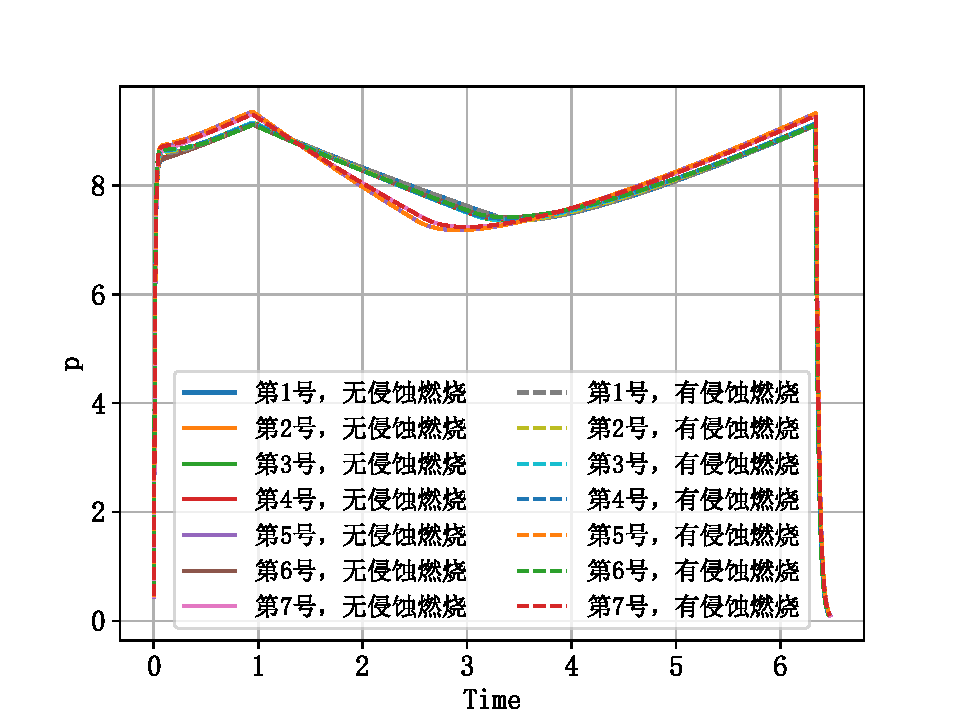
\includegraphics[width=0.89\linewidth]{双图全局总览.pdf}
    \caption{对比图}
    \label{fig:example}
  \end{figure}

\begin{figure}[!h]
    \centering
    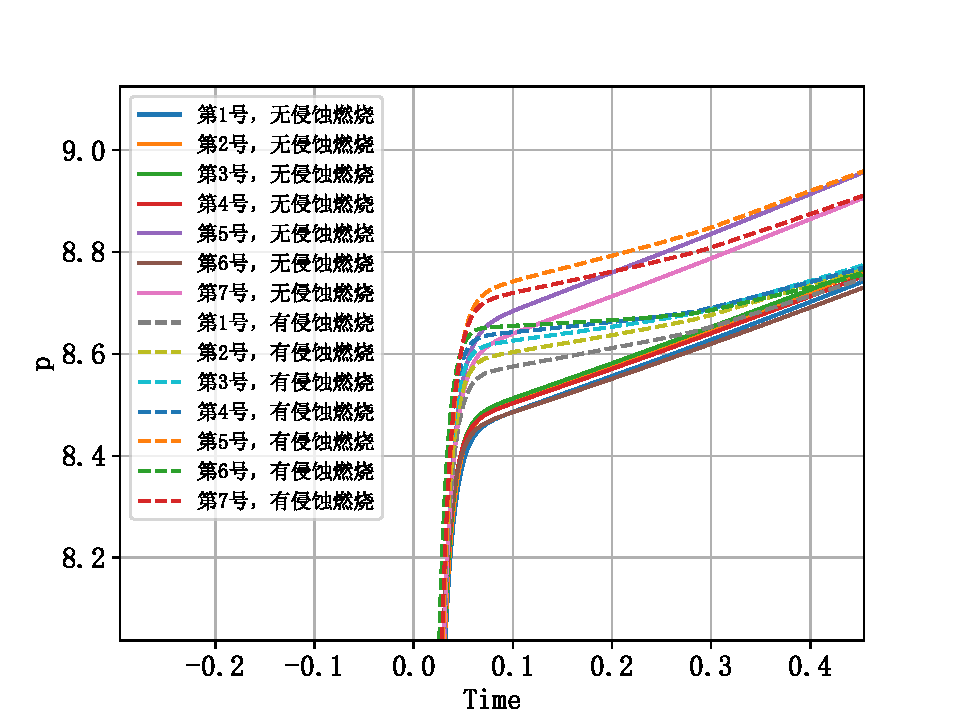
\includegraphics[width=0.89\linewidth]{双图局览左.pdf}
    \caption{对比图局部放大(左)}
    \label{fig:example}
  \end{figure}

\begin{figure}[!h]
    \centering
    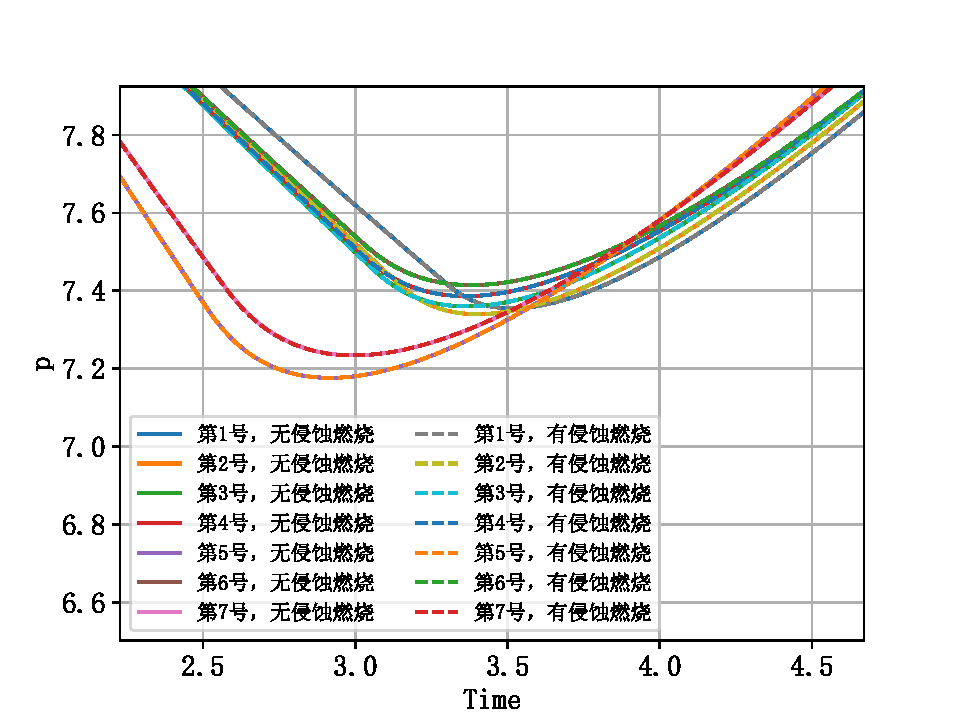
\includegraphics[width=1\linewidth]{双图局览中.pdf}
    \caption{对比图局部放大(中)}
    \label{fig:example}
  \end{figure}

  \begin{figure}[!h]
    \centering
    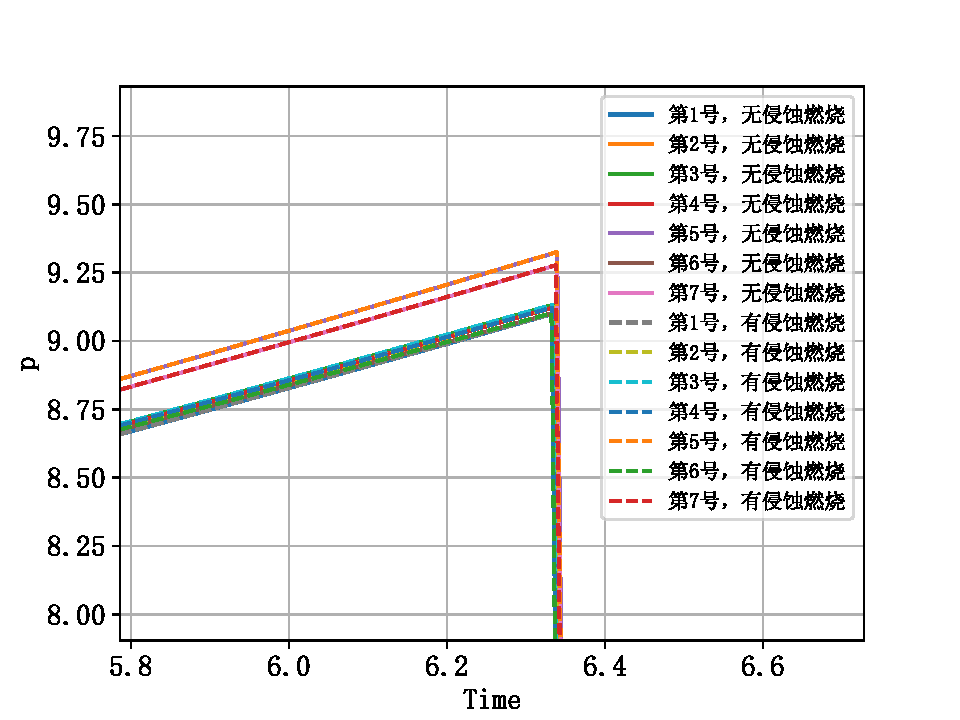
\includegraphics[width=1\linewidth]{双图局览右.pdf}
    \caption{对比图局部放大(右)}
    \label{fig:example}
  \end{figure}

\section{分析}
压强时间曲线的形状和燃烧面积时间变化曲线的形状吻合较好。

在燃烧室压强上升段,侵蚀燃烧$p-t$曲线初始爬升的更高,有益于爬升段。

除了初始阶段外,有侵蚀燃烧与无侵蚀燃烧$p-t$曲线几乎完全重合,说明侵蚀燃烧作用影响只发生在燃烧初始阶段对燃烧后期无影响。

有侵蚀燃烧效应产生的压力初始值影响不大,说明设计十分合理,降低了侵蚀燃烧对发动机壳体强度和工作可靠性的影响。

无论是否发生侵蚀燃烧,p-t图都是5号和7号接近,其他五组较为接近。

